\documentclass[spanish,letterpaper]{templates/uchile-tesis}

% Comandos especiales de esta tesis
%\newcommand{\mb}{\textit{microblogging}\xspace}
%\newcommand{\web}{Web\xspace}
%\newcommand{\tw}{\textit{Twitter}\xspace}
%\newcommand{\etal}{\textit{et. al.}\xspace}

% Portada - Variables
\facultad{Facultad de Ciencias Físicas y Matemáticas} 
\departamento{Departamento de Ciencias de la Computación}
\title{Comparación de algoritmos de extracción de skeleton}

\trabajoygrado{Tesis para optar al grado de Magíster en Ciencias de la Computación}

\author{Alejandro Manolete Lavado Abarzúa}

\profguia{Nancy Hitschfeld Kahler} %profesor guia
\profcoguia{Mauricio Cerda Villablanca} %profesor co-guia
\profint{Sr. ZZZ ZZZ ZZZ} %profesor integrante
\profinta{Sr. ZZ ZZ ZZ} %profesor integrante 2, generalemente no es necesario
\profintb{Sr. ZZZ ZZZ ZZZ} %profesor integrante 3, generalmente no es necesario
\proyecto{Financiado por el proyecto \#steffen}

\ciudad{Santiago} \pais{Chile} \monthpub{Diciembre} \yearpub{2017}

\begin{document}

% Lista de TODOS y FIXMES, no aparece si es que no hay nada que hacer
\listoftodos
\newpage

%% Portada
\maketitle

% Prefacio
\begin{preface}
% Resumen
\section{Resumen Ejecutivo}

% Pagina Optativa - Dedicatoria
\dedicatoria{Al cosmos}

% Pagina Optativa - Agradecimientos
\section{Agradecimientos}

\noindent Gracias a la tesis que me ha dado tanto

\noindent Me dio tres programas que cuando los abro

\noindent Perfecto distingo lo negro del blanco

\noindent Y en el esqueleto su aspecto delgado

\noindent Y en las magnitudes el pixel sobrando 

\noindent Gracias a la tesis que me ha dado tanto

\noindent Me ha dado 

\noindent Gracias a la tesis que me ha dado tanto

\noindent Me ha dado el olvido de lo investigado

\noindent 


\begin{flushright}
\makeatletter
	\@author
\makeatother
\end{flushright}

% Indice - General
\tableofcontents

% Indice - Tablas
\listoftables

% Indice - Figuras
\listoffigures

\end{preface}

% Introducción
\chapter{Introducción}
\label{ch:introduction}

\fillup{1}

\todo{todo 1} asdfasfsdfsadafs \missingref{me faltaría una ref!}.
\todo[inline]{todo 2}

% Algoritmos
\chapter{Definiciones y Notación}
\label{ch:defs}

El objetivo de este capítulo es presentar al lector las notaciones y conceptos que se usarán en los capítulos posteriores.

La inclusión de este capítulo se considera necesaria no .... En primer lugar, la topología digital es . En segundo lugar, con la esperanza de evitar la ambigüedad en las definiciones presente en la literatura de topología digital. Por ejemplo, algunos autores incluyen a los elementos dentro de sus vecindades \cite{cornea2007curve}, mientras que otros los dejan fuera \cite{lam1992thinning}.

Desde este capítulo en adelante, salvo cuando se indique algo distinto, la palabra \textit{algoritmo} se usa para referirse a un algoritmo que extrae el \textit{skeleton}.

\section{Estructura de los datos}

Los algoritmos implementados operan sobre imágenes binarias discretas. Esto quiere decir que su entrada y salida son matrices donde cada elemento vale 0 o 1. En adelante, el término \textit{imagen} se usa para referirse a esta representación matricial. En la literatura esta representación es calificada de implícita \cite{bloomenthal1997introduction}, porque las figuras son construidas a partir de un muestreo discreto.

El \textit{objeto} de una imagen es el conjunto de sus elementos que valen 1. El \textit{fondo} es el conjunto de sus elementos que valen 0. El \textit{skeleton} es el objeto de la imagen que un algoritmo produce como salida.

Si una imagen es de dos dimensiones (2D), los elementos que la constituyen se llaman \textit{píxeles}. Cuando es de tres dimensiones (3D), sus elementos se llaman \textit{vóxeles}. Los \textit{píxeles de objeto} son los píxeles que pertenecen al objeto; es decir, que valen 1. Los \textit{píxeles de fondo} son los píxeles que pertenecen al fondo, cuyo valor es 0. Los \textit{vóxeles de objeto} y \textit{vóxeles de fondo} se definen respectivamente de manera análoga. 

\todo{agregar ejemplo de imagen?}

\section{Conceptos de conectividad 2D}

\subsection{Relaciones de vecindad}
En una imagen 2D, cada píxel $p$ tiene exactamente 8 vecinos. Estos son los píxeles que rodean a $p$. Interpretando la imagen 2D como una grilla o celosía regular, donde cada píxel es un cuadrado, los vecinos de $p$ son los píxeles que comparten al menos un vértice con $p$. El conjunto de píxeles formado por $p$ y sus 8 vecinos se denomina la \textit{8-vecindad de $p$}. Es denotado $V_{8}(p)$. Además, se dice que $p$ es un \textit{8-vecino} de los demás elementos de $V_{8}(p)$.

Un tipo de adyacencia más estricto considera solo los vecinos de $p$ que comparten una arista (o, equivalentemente, dos vértices) con $p$. Desde un punto de vista matricial, estos son los vecinos de $p$ que están en la misma fila o columna que $p$. Exactamente 4 píxeles satisfacen esta condición. Entonces, se dice que estos píxeles son \textit{4-vecinos} de $p$. Unidos a $p$, forman la \textit{4-vecindad} de $p$, denotada $V_{4}(p)$. 

Es claro que $V_{4}(p) \subset V_{8}(p)$. Por consiguiente, si dos píxeles son 4-vecinos también son 8-vecinos. Además, todas las relaciones de vecindad son conmutativas. Si $p$ es $n$-vecino de $q$, entonces $q$ es $n$-vecino de $p$.

\subsection{Caminos y conectividad 2D} \label{conn2D}

Un \textit{8-camino} es una sucesión de píxeles $(p_{0}, p_{1}, \ldots, p_{k})$ que satisface dos condiciones. En primer lugar, todos sus píxeles son de objeto. En segundo lugar, cada uno de ellos, salvo el último, es 8-vecino del siguiente. Luego, se dice que dos píxeles $p$ y $q$ están \textit{8-conectados} si existe un 8-camino que empieza en $p$ y termina en $q$.

Análogamente, dos píxeles $p$ y $q$ están \textit{4-conectados} si existe un \textit{4-camino} que empieza en $p$ y termina en $q$.

Estas nociones de conectividad son fáciles de interpretar. Dos píxeles de objeto $p$ y $q$ están 8-conectados si es posible ir desde $p$ hasta $q$ moviéndose solamente entre 8-vecinos de valor 1. De igual modo, $p$ y $q$ están 4-conectados cuando esta secuencia de movimientos es posible sin efectuar movimientos diagonales.

\todo{agregar diagrama de las conectividades}

\section{Conceptos de conectividad 3D}

\subsection{Relaciones de vecindad}
Como se señaló anteriormente, una imagen 2D puede ser interpretada como una grilla regular, donde cada píxel es un cuadrado que comparte aristas y vértices con sus vecinos. Extendiendo esta misma noción, en una imagen 3D cada vóxel se puede interpretar como un cubo dentro de una grilla regular tridimensional. Entonces, cualquier vóxel $v$ puede ser ubicado en el centro de una subgrilla de $3\times3\times3$ vóxeles. El conjunto de vóxeles que pertenecen a esta subgrilla se denomina la \textit{26-vecindad de v}, porque en ella 26 vóxeles rodean a $v$. Se denota $V_{26}(v)$ y se dice que $v$ es \textit{26-vecino} de los demás elementos de $V_{26}(v)$. Todos los vóxeles de este conjunto, y solo ellos, comparten al menos un vértice con $v$ dentro de la grilla.

Un subconjunto importante de $V_{26}(v)$ son los vóxeles que comparten una cara con $v$. Como cada cubo de la grilla tiene 6 caras, existen 6 vóxeles con esta característica. El conjunto formado por estos vóxeles y $v$ se denomina la \textit{6-vecindad de v}, y se denota $V_6(v)$. Se dice que $v$ es \textit{6-vecino} de los demás vóxeles de $V_6(v)$.

Existe además un tercer tipo de adyacencia dentro de $V_{26}(v)$: los vóxeles que comparten alguna arista (o, equivalentemente, por lo menos dos vértices) con $v$. Esta condición significa excluir a los vecinos de $v$ que comparten exactamente 1 vértice con $v$. Gráficamente, quedan fuera los 8 vóxeles que ocupan las esquinas de la subgrilla de $3\times3\times3$ centrada en $v$. El conjunto conformado por $v$ y sus 18 vecinos restantes se denomina la \textit{18-vecindad de $v$}. Es denotado $V_{18}(v)$. Se dice que $v$ es \textit{18-vecino} de los demás elementos de este conjunto. 

Es conveniente destacar que $V_{6}(v) \subset V_{18}(v) \subset V_{26}(v)$. Por lo tanto, si dos vóxeles $v$ y $w$ son 6-vecinos, también son 18-vecinos y 26-vecinos.

\begin{figure}[ht]\centering
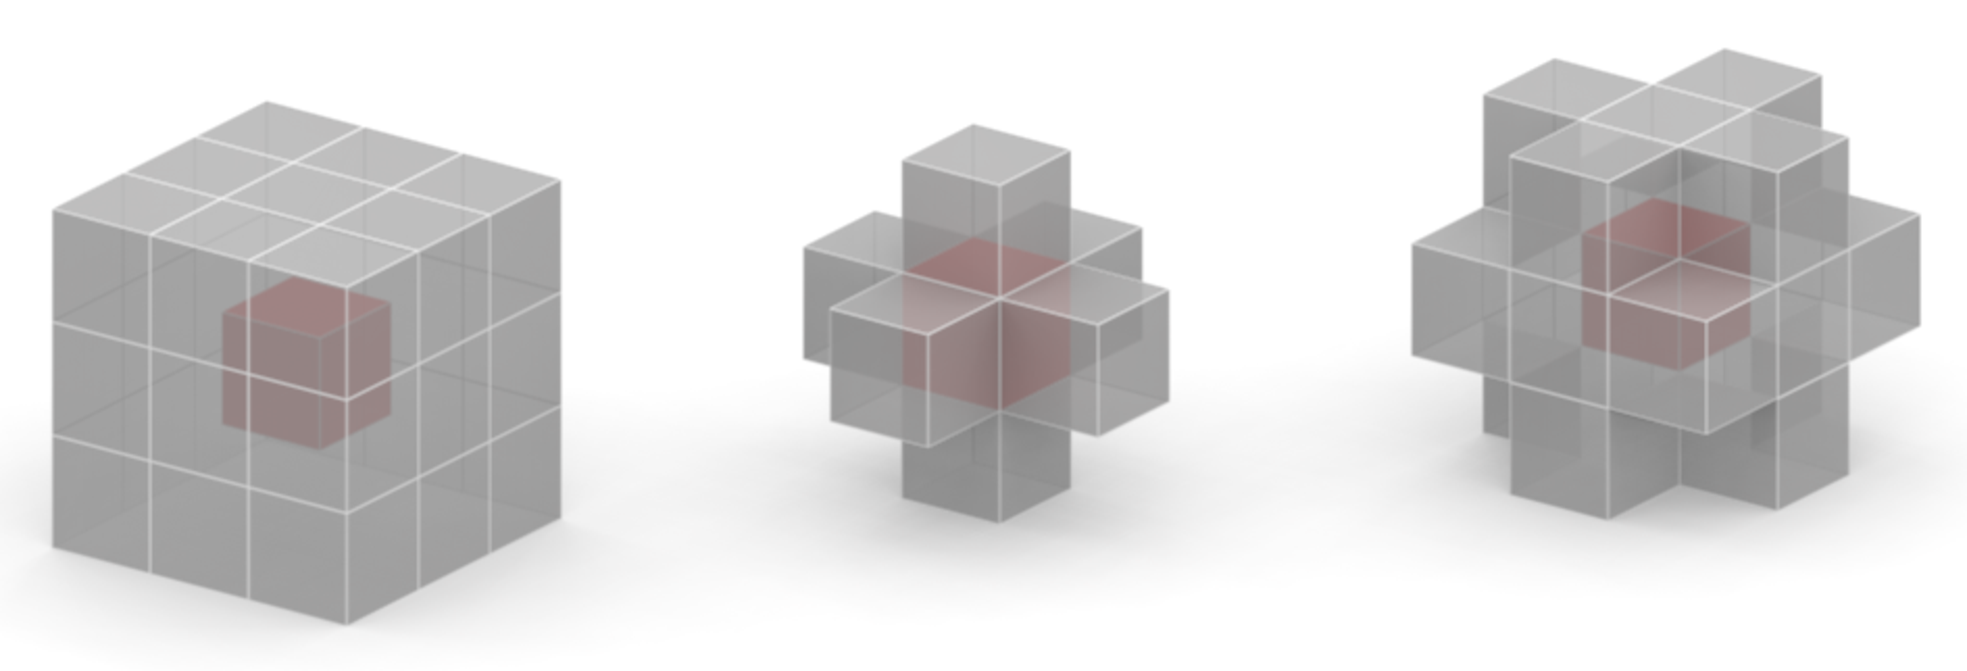
\includegraphics[width=0.8\linewidth]{images/3dneighborhoods}
\caption{Los 3 tipos de vecindades de un vóxel $v$: $V_{26}(v)$, $V_{6}(v)$ y $V_{18}(v)$.}
\label{fig:3dneighborhoods}
\end{figure}

\subsection{Caminos y conectividad 3D}

Al igual que para imágenes 2D, se define un tipo de camino por cada tipo de vecindad en una imagen 3D. Así, en imágenes 3D la definición de camino de la sección \ref{conn2D} se extiende para vóxeles, dando origen a \textit{26-caminos}, \textit{18-caminos} y \textit{6-caminos}.

Se dice que dos vóxeles $v$ y $w$ están \textit{26-conectados} si existe un 26-camino que empieza en $v$ y termina en $w$. De manera análoga, dos vóxeles pueden estar \textit{18-conectados} y \textit{6-conectados}.

\section{Conectividad en imágenes}

\subsection{Componentes conexas}

Dentro de una imagen, una \textit{componente $n$-conexa}, con $n \in \{4, 8\}$ si la imagen es 2D y $n \in \{6, 18, 26\}$ si es 3D, es un conjunto no vacío de píxeles o vóxeles que satisface dos condiciones. En primer lugar, cada elemento del conjunto está $n$-conectado con todos los demás. En segundo lugar, ningún elemento del conjunto está $n$-conectado con algún elemento fuera del conjunto. Es decir que, por ejemplo, dado un vóxel $v$, la componente $n$-conexa que contiene a $v$ es el conjunto maximal de vóxeles $n$-conectados a $v$. Si un conjunto no es $n$-conexo, se dice que es \textit{$n$-disconexo}.

\subsection{Condición básica para la preservación topológica} \label{ssec:fakehomotopy}

En la Sección \ref{sec:skelprops} se ha mencionado como requisito fundamental para la correctitud de un algoritmo el que la imagen de salida sea homotópica con la imagen de entrada. En la práctica, esta preservación topológica se traduce en que la imagen de salida debe tener el mismo número de componentes conexas de objeto y de fondo que la imagen de entrada \cite{saha1994topology}. Estos números dependen del tipo de conectividad que se escoja. Por ejemplo, la imagen de la Figura \ref{fig:8connectedcross} tiene 1 componente conexa de objeto y 1 componente conexa de fondo, independientemente a si se verifica la 4-conectividad o la 8-conectividad. Sin embargo, cambiar el valor del píxel marcado a 0 no altera el número de componentes 8-conexas, pero sí el de 4-conexas. Tras el cambio, la imagen presentaría 4 componentes 4-conexas de objeto y 2 componentes 4-conexas de fondo. Por lo tanto, un algoritmo que cambiara el valor del píxel rojo a 0 cumpliría con la propiedad homotópica si se usa la 8-conectividad y simultáneamente no la cumpliría si se usa la 4-conectividad.

\begin{figure}[ht]\centering
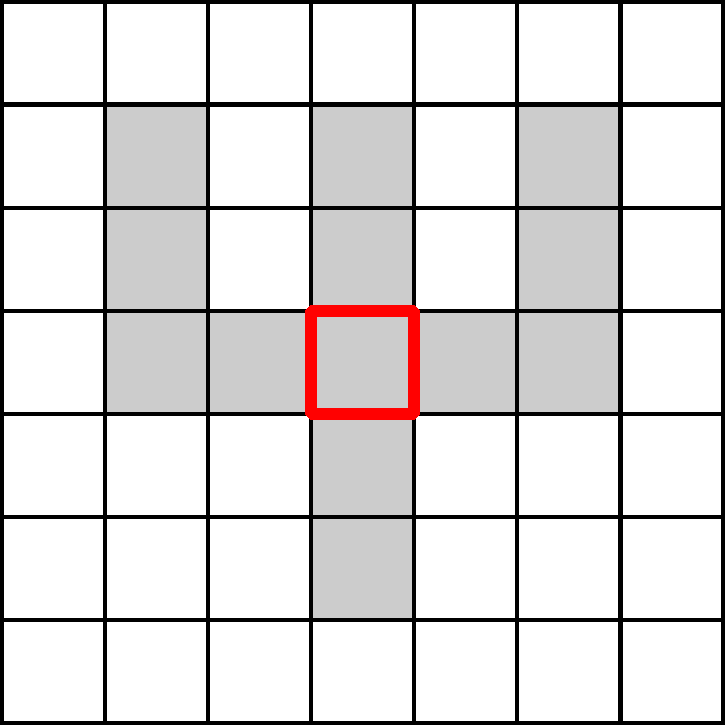
\includegraphics[width=0.35\linewidth]{images/8connectedcrossv2}
\caption{Removiendo el píxel marcado, objeto y fondo se mantienen 8-conexos, pero ambos se vuelven 4-disconexos.}
\label{fig:8connectedcross}
\end{figure}

\subsection{La paradoja del fondo} \label{ssec:paradox}

Casos como el anterior vuelven necesario convenir cuál tipo de conectividad se usará. Una posibilidad sería fijar la 8-conectividad para imágenes 2D y la 26-conectividad para imágenes 3D, argumentando que esto permitiría mayor libertad en la forma del \textit{skeleton}. Así, el \textit{skeleton} podría reproducir la forma del objeto original con mayor fidelidad.

Sin embargo, la Figura \ref{fig:diamong} ilustra una insatisfacción perceptual que resulta de elegir cualquier conectividad, descrita primero en \cite{duda1967graphical}. En esta imagen, tanto fondo como objeto son componentes 8-conexas, cuando la intuición sugiere que el objeto, un \textquotedblleft diamante\textquotedblright{}  8-conexo, debería dividir al fondo en un ``interior'' y un ``exterior''. De examinarse 4-conectividad, el diamante, siendo totalmente 4-disconexo, sí separaría al fondo en 2 componentes 4-conexas. El problema persiste en 3D. Basta pensar en una imagen donde el objeto sea el conjunto $V_{6}(v) - \{v\}$, para algún vóxel $v$ fijo. En esa imagen, tanto objeto como fondo serían 26-conexos, 18-conexos y 6-disconexos a la vez. Sin tratarse de un problema matemático, el que una componente disconexa separe componentes conexas, y viceversa, dificulta la comprensión de la topología digital \cite{rosenfeld1966sequential}.

\begin{figure}[ht]\centering
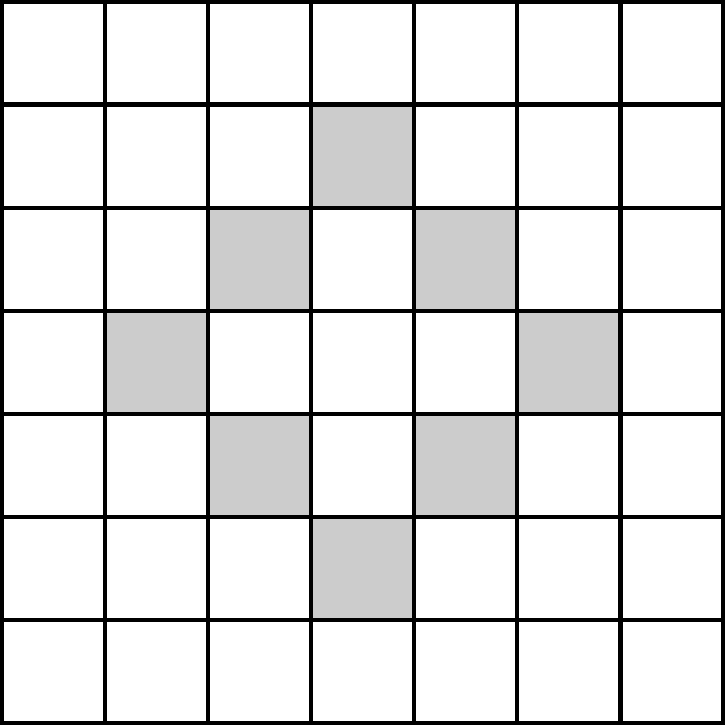
\includegraphics[width=0.35\linewidth]{images/diamong}
\caption{Imagen donde objeto y fondo son 8-conexos y 4-disconexos al mismo tiempo.}
\label{fig:diamong}
\end{figure}

La ambigüedad desaparece si se escoge algún tipo de conectividad para el objeto y uno diferente para el fondo. Para esta tesis se adopta la convención más común \cite{kong1989digital}. Se usará la 8-conectividad para el objeto y la 4-conectividad para el fondo en imágenes 2D. En imágenes 3D, se usará la 26-conectividad para el objeto y la 6-conectividad para el fondo. Siguiendo esta convención, es posible afirmar que en la Figura \ref{fig:diamong} el diamante conexo efectivamente desconecta al fondo.

\subsection{Búsqueda de componentes conexas}

Recorrer alguna componente conexa es un paso común dentro de los algoritmos implementados en esta tesis. Por lo general no es requisito etiquetar ni contar todas las componentes de una imagen (para lo cual existen algoritmos más apropiados \cite{thurfjell1992new}), sino recorrer alguna componente en particular a partir de un píxel o vóxel determinado. De acuerdo a \cite{vincent1991watersheds}, esto se consigue en tiempo lineal adaptando algún algoritmo de búsqueda en grafos para que recorra elementos de imágenes en lugar de nodos. La elección del algoritmo es arbitraria, porque el orden del recorrido no es relevante.

\begin{algorithm}
\caption{Recorrer una componente conexa por búsqueda en profundidad}
\label{alg:dfscc}
\begin{algorithmic}[1]
\Function{RecorrerCCporBEP}{$I$, $p$, $n$}
	\State\Comment{$I$ es la imagen, $p$ es el píxel o vóxel inicial, $n$ es la conectividad}
	\State $s \gets$ stack()
    \State $s$.push($p$)
    \While {$\neg$ $s$.empty()}
		\State $q \gets$ $s$.pop()
    	\If {$q$ no ha sido marcado como visitado}
    		\State marcar $q$ como visitado\Comment{Por lo general se hace algo con $q$ además de marcarlo}
			\ForAll{$r \in V_{n}(q) - \{q\}$}
            	\If {$val(q) = val(r)$} \label{valfirstuseever} \Comment{$val(x)$ es el valor de $x$ en la imagen, 0 o 1}
                  \State $s$.push($r$)
                \EndIf
    		\EndFor
        \EndIf
  	\EndWhile
\EndFunction
\end{algorithmic}
\end{algorithm}

El Algoritmo \ref{alg:dfscc}, implementado en esta tesis, corresponde a la búsqueda en profundidad \cite{hopcroft1973algorithm} adaptada a imágenes. En él, se comienza por ingresar en una pila todos los $n$-vecinos $n$-conectados a un nodo inicial $p$. Este proceso se repite recursivamente hasta vaciar la pila. La implementación iterativa para la recursión superó en eficiencia al uso de llamadas recursivas. Cabe señalar que la conectividad $n$ se podría inferir a partir del número de dimensiones de la imagen y de si $p$ es de objeto o de fondo, según la convención descrita en la sección anterior. Sin embargo, $n$ se explicita porque en ocasiones se querrá recorrer componentes conexas sin necesariamente obedecer esa convención.

\section{Criterios de preservación topológica}

\subsection{Noción de simplicidad}

Un píxel o vóxel de objeto es \textit{simple} si cambiar su valor a 0 (o \textit{eliminarlo}) no altera la topología de la imagen. Para saber si un elemento es simple, se podría calcular el número de componentes conexas en la imagen antes y después de eliminarlo, usando por ejemplo el Algoritmo \ref{alg:dfscc}, y revertir la eliminación si ese número cambia. Sin embargo, existen criterios más eficientes, capaces de determinar si un elemento es simple revisando únicamente su vecindad. A continuación se describen los métodos implementados para esta tesis.

\subsection{Simplicidad en 2D}

Precisando lo señalado anteriormente, un píxel de objeto es simple si eliminarlo no cambia el número de componentes 8-conexas de objeto ni el número de componentes 4-conexas de fondo. En este sentido, como fue demostrado en \cite{stefanelli1971some}, si un algoritmo elimina solamente píxeles simples efectivamente preserva la topología de la imagen. En otras palabras, un algoritmo que solamente elimine píxeles simples siempre cumplirá con la propiedad homotópica. \todo{poner codigos de colores en pixeles y estandarizar imagenes}

\begin{figure}[ht]\centering
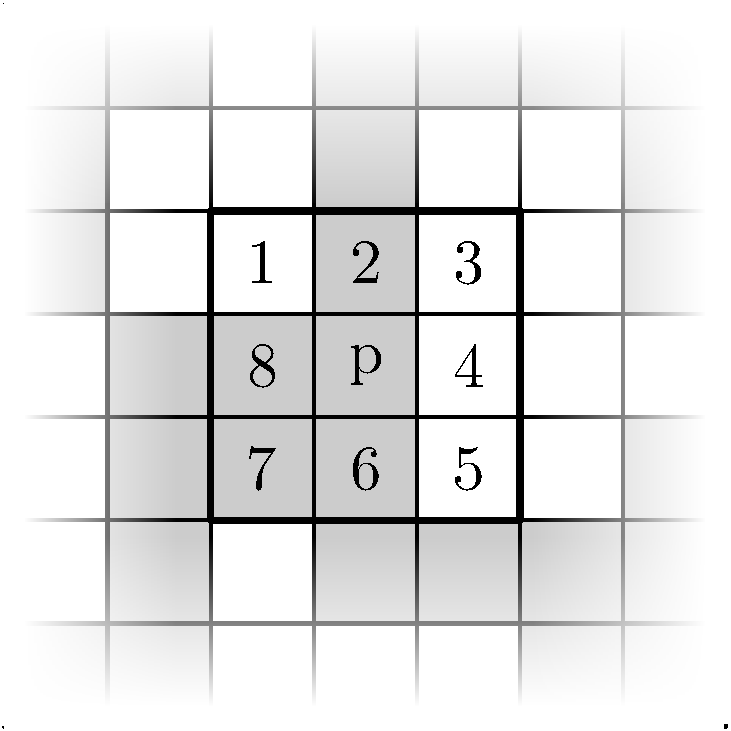
\includegraphics[width=0.35\linewidth]{images/2dsimpletestimageextract}
\caption{Numeración de la vecindad de $p$ para construir su grafo de vecindad.}
\label{fig:2dsimplen8}
\end{figure}

El criterio para determinar la simplicidad en imágenes 2D implementado en esta tesis es el que aparece en \cite{siddiqi2002hamilton}. Dado un píxel $p$, se numera su 8-vecindad como se muestra en la Figura \ref{fig:2dsimplen8}. Nótese que $p$ no se numera. El \textit{grafo de vecindad de} $p$ se construye situando primero un nodo sobre cada píxel de objeto numerado y luego una arista entre cada par de nodos situados sobre píxeles 8-vecinos entre sí. Si alguna de las 3-tuplas $(2, 3, 4)$, $(4, 5, 6)$, $(6, 7, 8)$ u $(8, 1, 2)$ corresponde a nodos del grafo, se elimina la respectiva arista diagonal $(2, 4)$, $(4, 6)$, $(6, 8)$ u $(8, 2)$. Con esto se remueven los posibles ciclos de largo 3.

\begin{figure}[ht]\centering
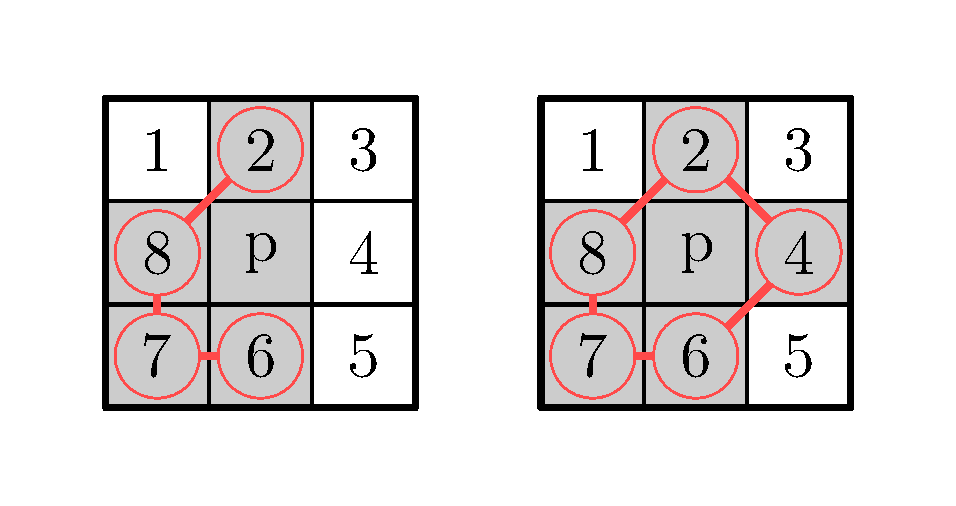
\includegraphics[width=0.6\linewidth]{images/2dsimpletestgraphcases}
\caption{Grafos de vecindad para dos píxeles distintos. En ambos casos la arista que conectaba los nodos 6 y 8 ha sido removida.}
\label{fig:2dsimpleexamples}
\end{figure}

Examinar las relaciones de adyacencia entre los nodos del grafo de vecindad de $p$ indica qué sucedería al eliminar $p$. Si la eliminación de $p$ desconectaría el objeto, el grafo de vecindad de $p$ es disconexo. Si la eliminación de $p$ originaría una componente de fondo (un ``agujero''), el grafo de vecindad de $p$ tiene un ciclo. Un grafo conexo sin ciclos es un árbol. Por lo tanto, se cumple el siguiente lema:

\begin{prop}
Un píxel $p$ es simple si su grafo de vecindad es un árbol.
\end{prop}

Un criterio directo para determinar si el grafo de vecindad es un árbol consiste en comprobar si su característica de Euler, el número de vértices menos el número de aristas, es igual a 1. La Figura \ref{fig:2dsimpleexamples} muestra ejemplos donde $p$ es simple y donde no.

\subsection{Simplicidad en 3D}

Además de componentes conexas, las imágenes 3D pueden presentar un elemento topológico adicional. La Figura \ref{fig:tunnelexample} ilustra un ejemplo. Difíciles de definir y encontrar \cite{svensson2003finding}, los  \textit{túneles} también deben considerarse al evaluar la preservación topológica de un algoritmo \cite{cornea2007curve}. Informalmente, un túnel es un agujero que atraviesa un objeto sin desconectarlo. Una definición formal de túnel puede encontrarse en \cite{kong1989digital2}, pero no es necesaria para esta tesis. Solo es preciso considerar que la eliminación de un vóxel puede originar un túnel, alterando con ello la topología de la imagen sin cambiar el número de componentes conexas. Por lo tanto, un algoritmo 3D satisfará la propiedad homotópica si el \textit{skeleton} que calcula preserva el número de componentes 26-conexas de objeto, el número de componentes 6-conexas de fondo y además el número de túneles de la imagen original \cite{Lieutier20041029}.

\begin{figure}[ht]\centering
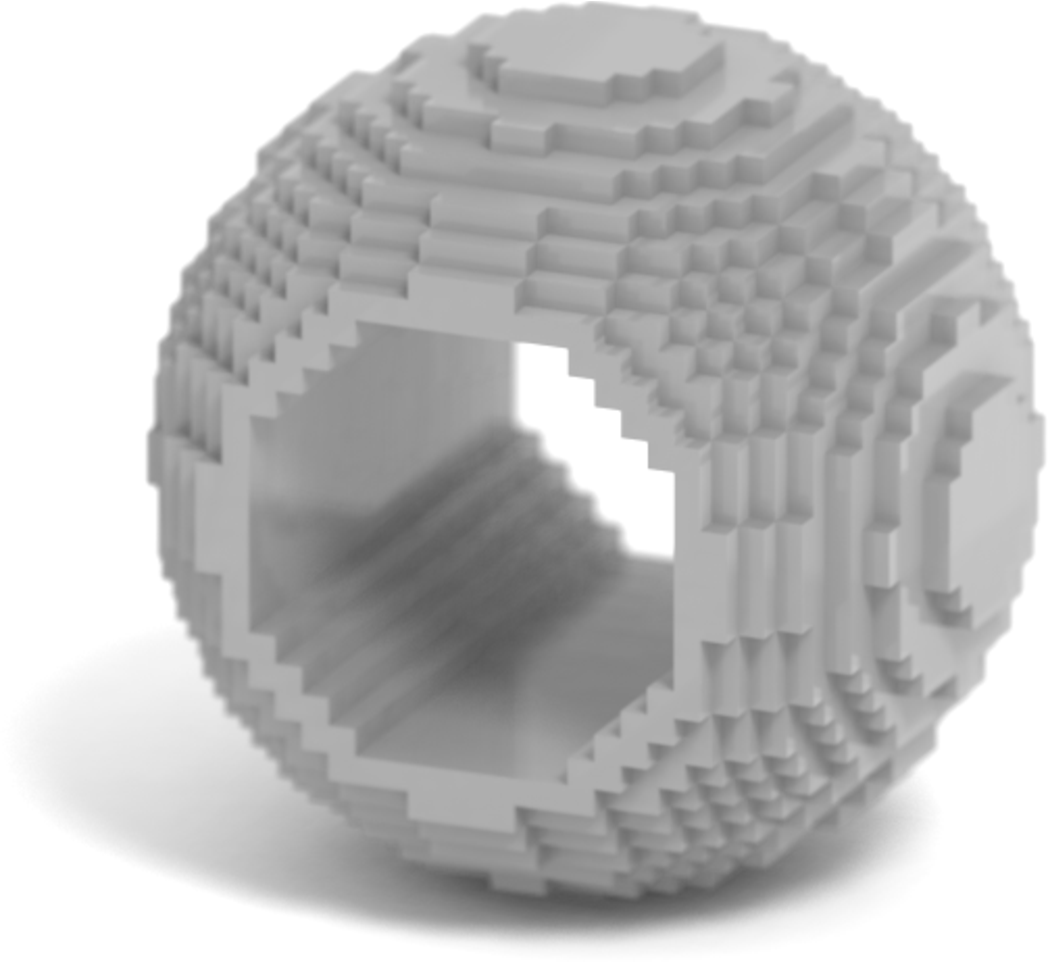
\includegraphics[width=0.4\linewidth]{images/tunnelexample}
\caption{Ejemplo de imagen 3D con un túnel.}
\label{fig:tunnelexample}
\end{figure}

Se han propuesto varios criterios para determinar la simplicidad de un vóxel \cite{kong1989digital2, tsao1981parallel, university1981three}. En esta tesis se utiliza la caracterización provista por Bertrand y Malandain \cite{bertrand1994new}. Esta caracterización comienza por definir dos números:

\begin{itemize}
\item $C(v)$ como el número de componentes 26-conexas de objeto en $V_{26}(v) - \{v\}$ y
\item $\bar{C}(v)$ como el número de componentes 6-conexas de fondo en $V_{18}(v) - \{v\}$ con algún vóxel 6-vecino a $v$.
\end{itemize}

Luego, se cumple el siguiente teorema:
\begin{theorem}
Un vóxel $v$ es simple ssi $C(v) = 1$ y $\bar{C}(v) = 1$.
\end{theorem}

Tener en cuenta la noción de punto  simple al diseñar un algoritmo basta para satisfacer la propiedad homotópica. Como se ha dicho antes, la topología podría conservarse con imponer la restricción de eliminar exclusivamente puntos simples. Sin embargo, esta estrategia no asegura en ninguna medida el resto de las propiedades del \textit{skeleton}. Los píxeles de los extremos de una línea, por ejemplo, son simples, pero eliminarlos significaría perder información de la forma de la figura (es más, la línea podría ser transformada en un punto aplicando sucesivamente este criterio). Por lo tanto, hace falta una noción adicional.

\begin{figure}[ht]\centering
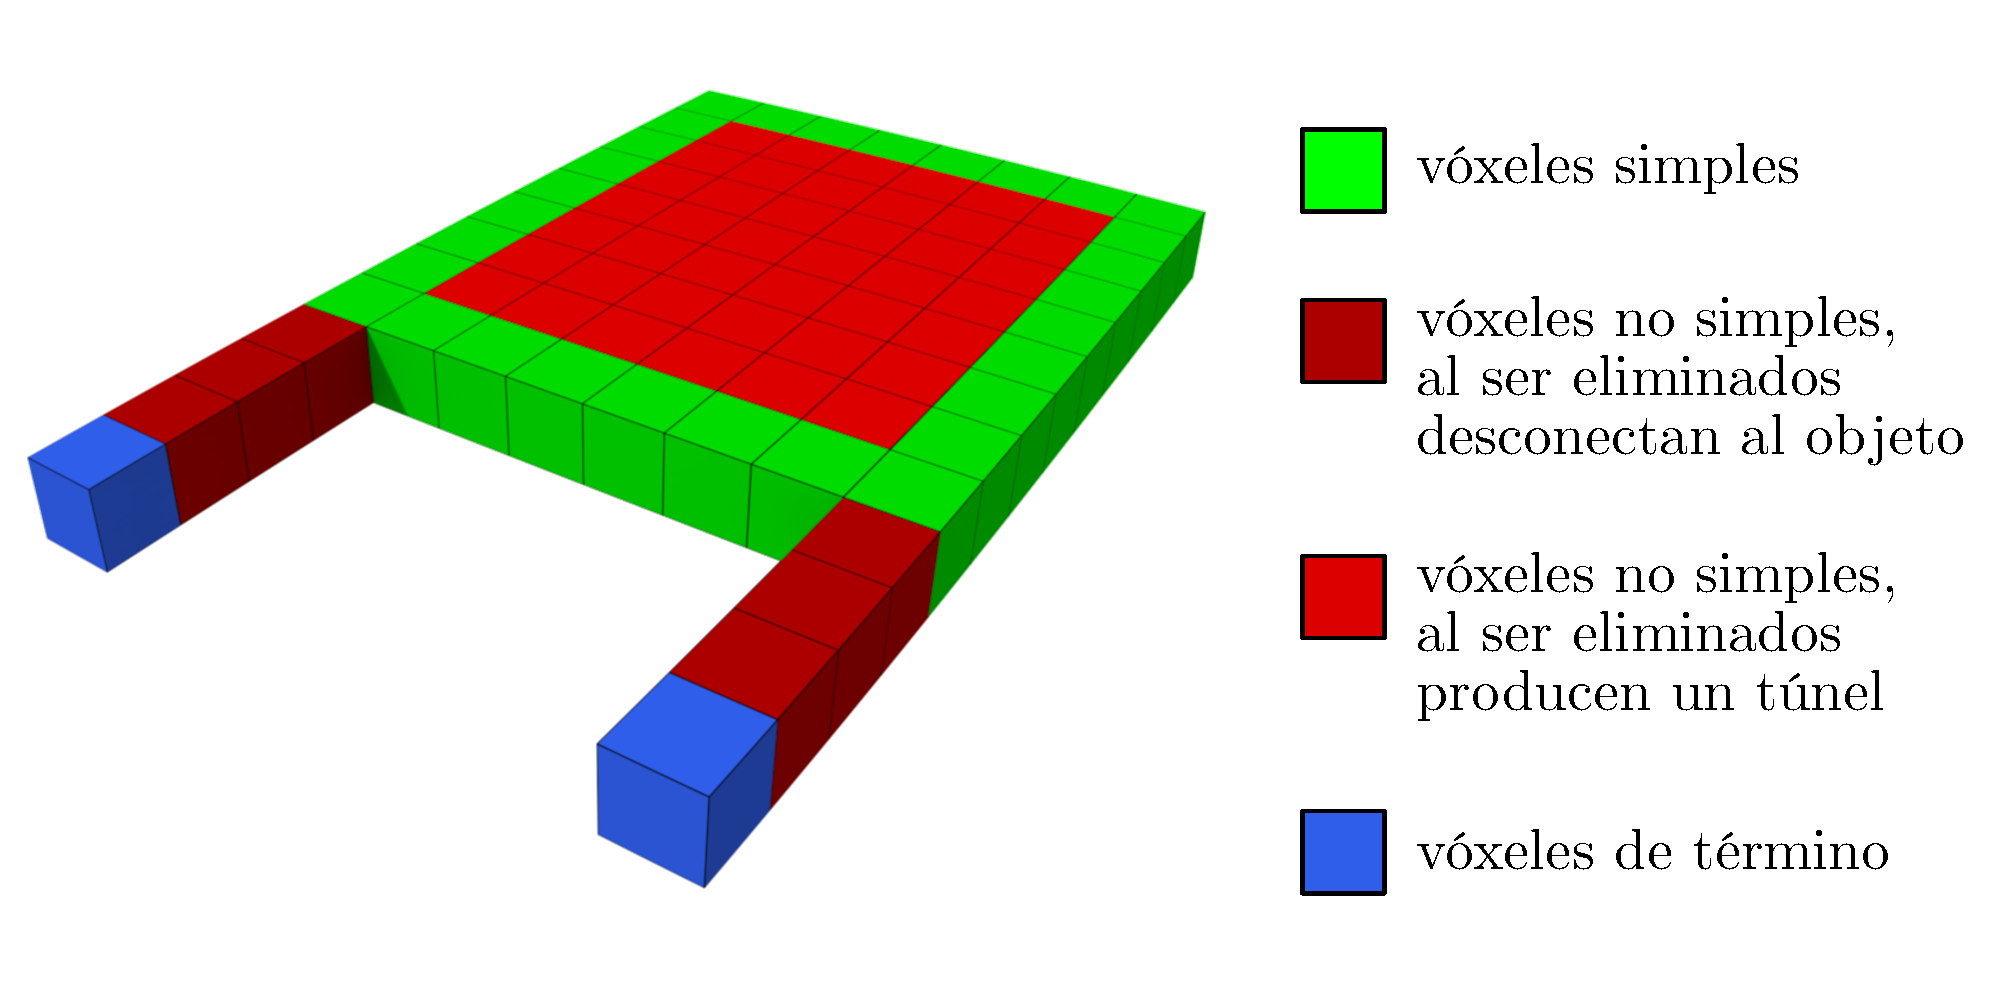
\includegraphics[width=0.7\linewidth]{images/voxel_types}
\caption{Principales tipos de vóxeles.}
\label{fig:voxeltypes}
\end{figure}

\subsection{Píxeles y vóxeles de término}

Un \textit{píxel de término} es un píxel de objeto que tiene exactamente 1 píxel de objeto adicional en su 8-vecindad. Similarmente, un \textit{vóxel de término} es un vóxel de objeto que tiene exactamente 1 vóxel de objeto adicional en su 26-vecindad.

El que un elemento sea de término significa que está en el extremo de una línea. En principio, todas las líneas son necesarias para que el \textit{skeleton} exprese la forma del objeto original con fidelidad, por lo que un algoritmo debería preservar todos los elementos de término. Sin embargo, algunas líneas pueden ser poco relevantes. Un algoritmo debe ser cuidadoso al decidir si un elemento de término debe ser eliminado.

\section{Nota sobre el preprocesamiento} \label{sec:noteInfinity}
Antes se señaló que, por ejemplo, en una imagen 2D cada píxel tiene exactamente 8 vecinos. No obstante, es claro que esta afirmación no se sostiene en la práctica. Las imágenes tienen dimensiones finitas en el computador, es decir que los píxeles de su contorno tienen menos de 8 vecinos (o menos de 26 vecinos para imágenes 3D). Para evitar complicaciones en el código debido a casos de este estilo, dentro de cada algoritmo las imágenes son preprocesadas, adosándoles una capa de píxeles de fondo como relleno. La forma común de referirse a esto es decir que se aplica un \textit{padding} de dimensión 1. Estos píxeles artificiales se ignoran cada vez que se recorre la imagen, y son removidos antes de producir la salida del algoritmo, restaurando así las dimensiones originales de la entrada.
\chapter{Skeletonización por Adelgazamiento Topológico Paralelo}
\label{ch:palagyi}

El primer algoritmo implementado para esta tesis fue presentado por Palágyi et al. en \cite{palagyi1999parallel}. Este algoritmo simula la metáfora del incendio de Blum eliminando vóxeles del contorno del objeto hasta transformarlo en el \textit{skeleton}. La secuencia de eliminación no es arbitraria, sino que está determinada por máscaras. Un vóxel es eliminado si su vecindad calza con alguna máscara, es decir, si satisface cierto patrón. En general, los algoritmos que siguen una estrategia similar son referidos como ''algoritmos de adelgazamiento topológico'', porque cada operación de eliminación va haciendo más delgado el objeto sin alterar su topología. En otras palabras, una condición mínima para las máscaras es que solamente vóxeles simples sean eliminados y se preserven los vóxeles de término.

Este algoritmo se dice además ''paralelo'' porque todos los vóxeles que calzan con cualquier máscara pueden ser eliminados simultáneamente. Sin embargo, a diferencia de los algoritmos de adelgazamiento ''totalmente paralelos'', las máscaras deben aplicarse varias veces en cada paso, rotadas en distintas direcciones. La mayoría de los algoritmos paralelos y totalmente paralelos usa 6 rotaciones, pero Este algoritmo en particular usa 12 rotaciones, o ''subiteraciones''.

\section{Fundamentos teóricos}



\subsection{La transformada \textit{hit-and-miss}}

\section{Visión general del algoritmo}

\algdef{SE}[DOWHILE]{Do}{doWhile}{\algorithmicdo}[1]{\algorithmicwhile\ #1} %do-while definicion jeje no se por que funciona

\begin{algorithm}[H]
\caption{Adelgazamiento topológico paralelo de Palágyi et al.}
\label{alg:thinning}
\begin{algorithmic}[1]
\Function{Adelgazamiento}{$I$}
	\State $masks \gets InitMasks()$
	\State $rotations \gets InitRotations()$
	\State $skel \gets I$
  	\Do
    	\State $prevSkel \gets skel$
    	\ForAll {$mask \in masks$}
        	\ForAll {$rotation \in rotations$}
            	\State $rotatedMask \gets rotate(mask, rotation)$
        		\State $skel \gets hitAndMiss(skel, rotatedMask)$
            \EndFor
        \EndFor
  	\doWhile{$prevSkel \neq skel$}
    \State \Return $skel$
\EndFunction
\end{algorithmic}
\end{algorithm}

En resumen, este algoritmo sencillamente aplica a la imagen original todas las máscaras, rotadas en cada una de las 12 rotaciones predefinidas, hasta que no se observen cambios.

\section{Las máscaras}
\chapter{Skeleton de Hamilton-Jacobi}
\label{ch:siddiqi}

La metáfora del incendio de Blum \cite{Blum:1967} dice que el \textit{skeleton} de un objeto se puede obtener encendiéndole fuego a toda su frontera simultáneamente. Luego, se asume que los frentes de llamas se propagan a una velocidad constante hacia el interior del objeto. Una vez que el fuego ha alcanzado todo el objeto, el \textit{skeleton} queda formado en los lugares donde dos frentes distintos se encontraron. En otras palabras, el \textit{skeleton} corresponde a los puntos de extinción, donde el fuego no pudo seguir avanzando por haberse encontrado consigo mismo. Estos puntos se conocen hoy en día como \textit{puntos de choque} \cite{leymarie2003three}.

Es posible simular directamente el frente de propagación de Blum como un flujo geométrico homogéneo \cite{kimmel1995skeletonization}. Sin embargo, enfrentar el problema específico de encontrar los puntos de choque (y por lo tanto, el \textit{skeleton}) permite simplificar los cálculos de varias maneras. Con ese propósito, los autores del algoritmo descrito en este capítulo recurrieron a herramientas de la mecánica lagrangiana.

\section{Fundamentos teóricos}
 
El desarrollo teórico subsecuente pertenece a la geometría diferencial. En consecuencia, la palabra \textit{objeto} ve alterado provisoriamente su significado dentro de esta sección. Los objetos 2D pasan a ser superficies cerradas y los objetos 3D pasan a ser volúmenes.

\subsection{Flujo de acortamiento de curvas}
Dado un objeto siendo atravesado por un frente de propagación, sea $\boldsymbol{C}(t)$ su frontera en el instante $t$. Es decir, $\boldsymbol{C}(t)$ es la frontera de la porción interior del objeto que en el instante $t$ todavía no ha sido alcanzada por el frente de propagación. $\boldsymbol{C}$ es una curva cerrada en 2D y una superficie cerrada en 3D. Además, $\boldsymbol{C}(0)$ es la frontera original del objeto. El movimiento del frente está dado por
\begin{equation}
\frac{\partial{\boldsymbol{C}}}{\partial{t}} = f\boldsymbol{n}
\end{equation}

\noindent
donde $f$ es la rapidez constante de propagación y $\boldsymbol{n}$ es el vector unitario normal interior a $\boldsymbol{C}$. Esta ecuación dice que $\boldsymbol{C}(t + \epsilon)$ se obtiene si todos los puntos de $\boldsymbol{C}(t)$ se mueven hacia el interior de $\boldsymbol{C}(t)$ con rapidez $f$ durante un tiempo $\epsilon$. En 2D es denominada \textit{flujo de acortamiento de curvas}. Su validez se sostiene para el caso 3D, donde describe la contracción de una superficie.

No existe un método analítico que sea capaz de detectar los puntos de choque directamente a partir de la ecuación (5.1), aunque sí es posible encontrarlos mediante una simulación numérica \cite{sethian1996fast}. Un enfoque más eficiente comienza por mostrar que esta ecuación en un caso particular de la \textit{ecuación de la eikonal}.

Sea $T$ un gráfico de la solución de la ecuación anterior. Es decir, $T$ es un campo escalar, donde cada paso en la evolución de $\boldsymbol{C}$ es asociado con el instante cuando ese paso tiene lugar. En otras palabras
\begin{equation}
T(\boldsymbol{C}(t)) = t.
\end{equation}

\noindent
Tomando la derivada con respecto al tiempo
\begin{equation}
\frac{d}{dt}T(\boldsymbol{C}(t)) = 1
\end{equation}
\begin{equation}
\frac{\partial T}{\partial \boldsymbol{C}}\cdot\frac{\partial \boldsymbol{C}}{\partial t} = 1
\end{equation}
\begin{equation}
\nabla T\cdot\frac{\partial \boldsymbol{C}}{\partial t} = 1.
\end{equation}

\noindent
Sustituyendo $\frac{\partial \boldsymbol{C}}{\partial t}$ usando la ecuación (5.1),
\begin{equation}
\nabla T\cdot f\boldsymbol{n} = 1
\end{equation}
\begin{equation}
||\nabla T|| f = 1.
\end{equation}

\noindent
Teniendo la ecuación (5.7) se afirma que $T$ satisface la \textit{ecuación de la eikonal}, un concepto fundamental de la óptica geométrica \cite{luneburg1964mathematical}.

A continuación se presenta una breve introducción a algunos conceptos de mecánica y óptica, necesarios para comprender la solución de esta ecuación, con los cuales el lector de computación podría no estar familiarizado. El objetivo es mostrar la relación existente entre las ecuaciones de la eikonal y la de Hamilton-Jacobi, que da nombre a este algoritmo. Las principales referencias para las siguientes subsecciones son los libros de Shankar \cite{shankar2012principles} y Arnold \cite{arnol2013mathematical}.

\subsection{Introducción a la mecánica lagrangiana}

Una partícula se encuentra en el eje horizontal $x$. Más precisamente, está posicionada sobre el punto $x_0$ en el instante $t_0$. Luego, sobre ella actúa un potencial (o fuerza) horizontal $V(x)$. Finalmente, debido a la acción de este potencial, en el instante $t_f$ se ha movido a la posición $x_f$. ¿Qué determina que su movimiento haya sido rectilíneo, a lo largo del eje $x$? ¿Por qué la partícula no escogió otro camino (por ejemplo, una curva) para llegar a $x_f$?

De acuerdo a la formulación lagrangiana, el movimiento de la partícula está restringido por el \textit{principio de mínima acción}. La \textit{acción} de cada posible camino $x(t)$ se define como
\begin{equation}
S[x(t)] = \int_{t_0}^{t_f} \! \mathcal{L}(x, \dot{x}) \, \mathrm{d}t
\end{equation}

\noindent
donde $\mathcal{L}$ es una función llamada \textit{lagrangiano}, cuyo valor es la diferencia entre las energías cinética y potencial de la partícula. El lagrangiano normalmente depende de la velocidad y la posición, que a su vez dependen del tiempo. Como es costumbre en mecánica, se usa la notación de Newton para la diferenciación: $\dot{x}$ indica la derivada de la posición con respecto al tiempo. Además, los paréntesis cuadrados se usan para indicar que $S$ es un \textit{funcional}, es decir, que depende de todo el camino $x(t)$ y no del valor de $x$ en algún instante $t$. El principio de mínima acción dice que la partícula clásica escogerá el camino $x_{cl}(t)$ que minimice $S$.

En general, como se demuestra en \cite{shankar2012principles}, el lagrangiano para el camino $x_{cl}(t)$ satisface la \textit{ecuación de Euler-Lagrange}
\begin{equation}
\frac{d}{dt} \frac{\partial\mathcal{L}}{\partial \boldsymbol{\mathrm{\dot{q}}}} - \frac{\partial\mathcal{L}}{\partial\boldsymbol{\mathrm{q}}} = 0,
\end{equation}

\noindent
donde $\boldsymbol{\mathrm{q}} = (q_1, q_2,... ,q_n)$ representa el conjunto de $n$ coordenadas independientes (o \textit{grados de libertad}) que determinan la posición de la partícula, y $\boldsymbol{\mathrm{\dot{q}}} = (\dot{q_1}, \dot{q_2},... , \dot{q_n})$ su velocidad. La ecuación (5.9) es central en mecánica, pues permite obtener las ecuaciones del movimiento simplemente derivando el lagrangiano.

La ecuación de Euler-Lagrange es un ejemplo para demostrar que las ecuaciones de la mecánica lagrangiana se sostienen para un sistema de coordenadas arbitrario. Sin embargo, en el contexto de esta tesis bastará con $\boldsymbol{\mathrm{q}} = (x, y, z)$.

\subsection{El formalismo hamiltoniano}

La mecánica hamiltoniana es una reformulación de la mecánica lagrangiana. Como se señaló anteriormente, en la mecánica lagrangiana las ecuaciones del movimiento derivan del lagrangiano $\mathcal{L}(\boldsymbol{\mathrm{q}}, \boldsymbol{\dot{\mathrm{q}}})$, el cual depende de la posición y la velocidad. En la mecánica hamiltoniana, en cambio, las ecuaciones del movimiento se obtienen a partir del \textit{hamiltoniano} $\mathcal{H}(\boldsymbol{\mathrm{q}}, \boldsymbol{\mathrm{p}})$, que depende de la posición y los \textit{momentos}. Estos últimos son cantidades que originalmente se derivan del lagrangiano:
\begin{equation}
\boldsymbol{\mathrm{p}} = \frac{\partial\mathcal{L}}{\partial\boldsymbol{\dot{\mathrm{q}}}}.
\end{equation}

\noindent
Sin embargo, la \textit{transformada de Legendre} permite transformar el lagrangiano $\mathcal{L}$ en el hamiltoniano $\mathcal{H}$ mediante la sencilla equivalencia
\begin{equation}
\mathcal{H}(\boldsymbol{\mathrm{q}}, \boldsymbol{\mathrm{p}}) = \boldsymbol{\mathrm{p}} \cdot \boldsymbol{\mathrm{\dot{q}}} - \mathcal{L}(\boldsymbol{\mathrm{q}}, \boldsymbol{\dot{\mathrm{q}}}).
\end{equation}

\noindent
Tomando la derivada parcial con respecto a $\boldsymbol{\mathrm{p}}$ se comprueba que esta transformada efectivamente invierte los roles de $\boldsymbol{\mathrm{p}}$ y $\boldsymbol{\dot{\mathrm{q}}}$: ahora la velocidad $\boldsymbol{\dot{\mathrm{q}}}$ se deriva del hamiltoniano,
\begin{equation}
\boldsymbol{\dot{\mathrm{q}}} = \frac{\partial \mathcal{H}}{\partial \boldsymbol{\mathrm{p}}}.
\end{equation}

\noindent
Además, es posible usar la ecuación (5.10) para reemplazar $\frac{\partial \mathcal{L}}{\partial \boldsymbol{\dot{\mathrm{q}}}}$ por $\boldsymbol{\mathrm{p}}$ en la ecuación (5.9). Al mismo tiempo, tomar la derivada parcial con respecto a $\boldsymbol{\mathrm{q}}$ en la ecuación (5.11) resulta en $-\frac{\partial \mathcal{L}}{\partial \boldsymbol{\mathrm{q}}} = \frac{\partial \mathcal{H}}{\partial \boldsymbol{\mathrm{q}}}$. Incorporando ambos resultados a la ecuación (5.9) se obtiene
\begin{equation}
\boldsymbol{\dot{\mathrm{p}}} = -\frac{\partial \mathcal{H}}{\partial \boldsymbol{\mathrm{q}}}.
\end{equation}

\noindent
Las ecuaciones (5.12) y (5.13) se conocen como las \textit{ecuaciones canónicas de Hamilton}. 

\subsection{}

\section{Visión general del algoritmo}

\begin{algorithm}[H]
\caption{Extracción del \textit{skeleton} de Hamilton-Jacobi}
\label{alg:hjskel}
\begin{algorithmic}[1]
\Function{SkeletonDeHamiltonJacobi}{$I$, $\tau$}
	\State $D \gets TDE(I)$
    \State $\nabla D \gets Gradiente(D)$
    \State $\mathcal{F} \gets FlujoEmergentePromedio(\nabla D)$
    \State $h \gets maxHeap()$
    \ForAll {$p$ en el borde de $I$}
    	\If {$p$ es simple}
        	\State $h.insert(p, \mathcal{F}(p))$ \Comment $p$ se inserta con el flujo como clave de ordenamiento
        \EndIf
    \EndFor
    \While {$h.size() > 0$}
    	\State $p \gets h.extractMax()$
        \If {$p$ es simple}
        	\If {$p$ no es punto de término o $\mathcal{F}(p) > \tau$}
            	\State Remover $p$ de $I$
                \ForAll {$q \in V_{26}(p)$} 
                	\If {$q$ es simple}
                    	\State $h.insert(q, \mathcal{F}(p))$
                    \EndIf
                \EndFor
            \Else
            	\State Marcar $p$ como no removible
            \EndIf
        \EndIf
    \EndWhile
    \State \Return $I$
\EndFunction
\end{algorithmic}
\end{algorithm}

\section{Detalle de la implementación}


\chapter{Skeletonización basada en distancia}
\label{ch:arcelli}

El tercer algoritmo implementado para esta tesis fue presentado por Arcelli et al. en \cite{arcelli2011distance}. Este algoritmo  de los otros dos porque utiliza la segunda definición del \textit{skeleton} presentada en el Capítulo \ref{ch:introduction}. En lugar de incendiar los objetos, el \textit{skeleton} es calculado a partir de los centros de discos o bolas maximales inscritas en el objeto.

El algoritmo cuya implementación se detalla en esta capítulo fue concebido para calcular el \textit{skeleton} de imágenes 3D. Para adquirir familiaridad con las técnicas usadas, se comenzó por implementar el algoritmo para imágenes 2D basado en discos maximales que aparece en \cite{di1996skeletonization}. Este algoritmo 2D calcula el \textit{skeleton} siguiendo principios parecidos al algoritmo 3D de este capítulo, pero su enfoque en imágenes bidimensionales le concede una relativa sencillez. En los anexos se han dedicado unas palabras a esa versión. La principal diferencia con la versión 3D está en la detección de puntos de bifurcación. No existe un equivalente para vóxeles del número de cruce de Hilditch \cite{hilitch1969linear}.

\section{Fundamentos teóricos}

\subsection{Transformadas de distancia}

Una \textit{transformada de distancia} de una imagen es un mapeo donde a cada píxel o vóxel de objeto se le asigna la distancia al píxel o vóxel de fondo más cercano. Los píxeles o vóxeles de fondo se mapean al valor constante 0 \footnote{A veces los elementos de fondo son mapeados a otros valores, como por ejemplo a $\infty$, pero para los algoritmos de esta tesis se usa siempre 0.}. En otras palabras, la transformada de distancia es una matriz con las mismas dimensiones que su imagen correspondiente. Si un elemento de la imagen vale 0, en su mismo índice dentro de la transformada de distancia aparecerá un 0. Si un elemento de la imagen vale 1, en su mismo índice dentro de la transformada de distancia aparecerá algún valor positivo que indique la distancia entre ese elemento y el elemento con valor 0 más cercano. Estos valores positivos dependerán de cómo se mida la distancia entre dos elementos.

Fue necesario esbozar el concepto de transformada de distancia para explicar el algoritmo del Capítulo \ref{ch:siddiqi}. Dentro de ese algoritmo, el cálculo de la transformada de distancia euclidiana era el primer paso para el cálculo del \textit{skeleton}. Las operaciones subsecuentes eran de carácter global. En contraste, la métrica euclidiana no es adecuada para determinar localmente si un vóxel corresponde al centro de una bola maximal. La transformada de distancia euclidiana busca ser exacta, por lo que no impone ninguna restricción para los valores que corresponden a vóxeles vecinos \cite{borgefors1991euclidean}. A pesar de esto, se han propuesto algunos algoritmos que la usan, como \cite{remy2003look}, basado en tablas de consulta con todos los valores posibles.

El algoritmo de este capítulo usa una transformada más amigable en el sentido anterior. Es parte de la familia de transformadas de distancia que se describe a continuación.

\subsection{La transformada de distancia <3,4,5>}

Una \textit{transformada de distancia con pesos} 3D es una transformada de distancia donde la distancia entre dos vóxeles es una constante que depende de su relación de vecindad. Se denota $\langle d_c,d_a,d_v \rangle$, donde $d_c$ es la distancia entre dos vóxeles que comparten una cara, $d_a$ es la distancia entre dos vóxeles que comparten una arista y $d_v$ es la distancia entre dos vóxeles que comparten un vértice. Para imágenes 2D se definen y denotan de manera equivalente.

La idea básica de las transformadas de distancia con pesos es aproximar la transformada de distancia euclidiana, simplificando al mismo tiempo los cálculos. La transformada de distancia con pesos que interesa para este algoritmo es la $\langle 3,4,5 \rangle$. 12\% 

\subsection{Centros de bolas maximales en la transformada de distancia <3,4,5>}

\subsection{El \textit{skeleton} como lugar geométrico}

Hablar del skeleton como el lugar geométrico del centro de las cbm y por que la 345 es mejor que le euclidiana.

12 por ciento de diferencia con la euclidiana \cite{borgefors1996digital}

\section{Visión general del algoritmo}

\begin{algorithm}
\caption{Skeletonización basada en distancia}
\label{alg:ddskel}
\begin{algorithmic}[1]
\Function{SkeletonizacionBasadaEnDistancia}{$I$, $\theta_1$, $\theta_2$}
	\State $td \gets TD345(I)$
    \State $cbm \gets ExtraerCBM(td)$
    \State $anclas \gets Filtrar(cbm)$
    \State $pss\_casi\_delgado \gets ErosionarYConectar(anclas)$
    \State $pss\_delgado \gets Adelgazar(pss\_casi\_delgado)$
    \State $pss \gets Podar(pss\_delgado, \theta_1, \theta_2)$ \label{ddprune1}
    \State $vc \gets ClasificarVoxeles(pss)$
    \State $tdd \gets TD345Delimitada(pss, vc)$
    \State $cbm\_pss \gets ExtraerCBM(pss, tdd)$
    \State $anclas\_pss \gets Filtrar(cbm\_pss)$
    \State $skeleton\_casi\_delgado \gets Erosionar(PSS, anclas\_pss)$
    \State $skeleton \gets Adelgazar(skeleton\_casi\_delgado)$
    \State $skeleton \gets Podar(skeleton, \theta_1, \theta_2)$ \label{ddprune2}
    \State \Return $skeleton$
\EndFunction
\end{algorithmic}
\end{algorithm}

Este algoritmo tiene muchos pasos. En la siguiente sección se detalla cada línea del pseudocódigo anterior.

\section{Descripción detallada de la implementación}

\subsection{Parámetros}

\begin{algorithm}[H]
\addtocounter{algorithm}{-1}
\caption{Parte 1}
\begin{algorithmic}[1]
\Function{SkeletonizacionBasadaEnDistancia}{$I$, $\theta_1$, $\theta_2$}
\algstore{bkbreak}
\end{algorithmic}
\end{algorithm}

Además de la imagen de entrada $I$, este algoritmo recibe los parámetros numéricos $\theta_{1}$ y $\theta_{2}$, que permiten calibrar el nivel de detalle del \textit{skeleton}. Puede observarse que ambos parámetros aparecen en las líneas \ref{ddprune1} y \ref{ddprune2} del pseudocódigo. Se trata de umbrales que determinan la eliminación de ramas poco significativas. Su significado se detalla  en la Sección \ref{ssec:prune1}, donde se describe la primera poda del \textit{skeleton}.

\subsection{Cálculo de la transformada de distancia <3,4,5>}

\begin{algorithm}[H]
\caption{Parte 2}
\begin{algorithmic}[1]
\algrestore{bkbreak}
\State $TD \gets TD345(I)$
\algstore{bkbreak}
\end{algorithmic}
\end{algorithm}

Para calcular la transformada $<3,4,5>$ se implementó el algoritmo descrito en \cite{borgefors1996digital}. Este algoritmo permite calcular cualquier transformada de distancia con pesos en tiempo lineal respecto al número de vóxeles de la imagen. La imagen es recorrida dos veces, propagando los costos mínimos desde esquinas opuestas en cada pasada. En siguiente pseudocódigo se muestra este algoritmo.

\begin{algorithm}[H]
\caption{Cálculo de la transformada de distancia $<3,4,5>$}
\label{alg:ddskel}
\begin{algorithmic}[1]
\Function{TD345}{$I$}
	\State $td \gets Ceros(I)$
	\For{$i \gets 1, filas$} \Comment{Recorrido hacia adelante}
	\For{$j \gets 1, columnas$}
	\For{$k \gets 1, capas$}
    	\If{$I_{i,j,k} = 1$}
        	\State $td_{i,j,k} \gets \min\limits_{(p,q,r) \in V_F}{td_{p,q,r} + d_n}$
        \EndIf
    \EndFor
    \EndFor
    \EndFor
	\For{$i \gets filas, 1$} \Comment{Recorrido hacia atrás}
	\For{$j \gets columnas, 1$}
	\For{$k \gets capas, 1$}
    	\If{$I_{i,j,k} = 1$}
        	\State $td_{i,j,k} \gets \min\limits_{(p,q,r) \in V_B}{td_{p,q,r} + d_n}$
        \EndIf
    \EndFor
    \EndFor
    \EndFor
    \State $ReemplazarValoresEquivalentes(td)$
    \State \Return $td$
\EndFunction
\end{algorithmic}
\end{algorithm}

El primer recorrido parte desde la esquina donde comienzan los índices en la implementación. Para cada vóxel de objeto $v$, $V_F(v)$ es el subconjunto ya recorrido de $V_{26}(v)$. $td(v)$ se calcula como el mínimo de tomar los valores de $td$ para ese conjunto y sumarles el peso $d_n$ correspondiente a la distancia local; por ejemplo, hay que sumar 5 a los vecinos que compartan solo un vértice con $v$. El segundo recorrido se efectúa en orden inverso. La única diferencia con el primer recorrido es que $V_B(v)$ contiene además el valor calculado para $v$ en el primer recorrido. Es decir, teniendo el largo del camino encontrado en el primer recorrido, el segundo recorrido verifica si existía un camino más corto partiendo desde el lado opuesto de la imagen.

Por último, la función $ReemplazarValoresEquivalentes()$ del final del algoritmo simplemente sustituye todos los valores 3 de la transformada por 1. Este reemplazo permite la identificación correcta de máximos locales cercanos a los bordes \cite{arcelli1988finding}.

\subsection{Extracción de CBM}

La transformada de distancia euclidiana

\begin{algorithm}[H]
\caption{Parte 3}
\begin{algorithmic}[1]
\algrestore{bkbreak}
\State $CBM \gets ExtraerCBM(I)$
\algstore{bkbreak}
\end{algorithmic}
\end{algorithm}



\subsection{Obtención de puntos ancla para el \textit{skeleton}}

\begin{algorithm}[H]
\caption{Parte 4}
\begin{algorithmic}[1]
\algrestore{bkbreak}
\State $anclas \gets Filtrar(CBM)$
\algstore{bkbreak}
\end{algorithmic}
\end{algorithm}

\subsection{Obtención del PSS casi delgado}

\begin{algorithm}[H]
\caption{Parte 5}
\begin{algorithmic}[1]
\algrestore{bkbreak}
\State $PSSCasiDelgado \gets ErosionarYConectar(anclas)$
\algstore{bkbreak}
\end{algorithmic}
\end{algorithm}

\subsection{Adelgazamiento del PSS}

\begin{algorithm}[H]
\caption{Parte 6}
\begin{algorithmic}[1]
\algrestore{bkbreak}
\State $PSSDelgado \gets Adelgazar(PSSCasiDelgado)$
\algstore{bkbreak}
\end{algorithmic}
\end{algorithm}

\subsection{Poda del PSS} \label{ssec:prune1}

\begin{algorithm}[H]
\caption{Parte 7}
\begin{algorithmic}[1]
\algrestore{bkbreak}
\State $PSS \gets Podar(PSSDelgado, \theta_1, \theta_2)$ \label{ddprune1}
\algstore{bkbreak}
\end{algorithmic}
\end{algorithm}

\subsection{Clasificación de vóxeles del PSS}

\begin{algorithm}[H]
\caption{Parte 8}
\begin{algorithmic}[1]
\algrestore{bkbreak}
\State $VC \gets ClasificarVoxeles(PSS)$
\algstore{bkbreak}
\end{algorithmic}
\end{algorithm}

\subsection{Cálculo de la transformada de distancia <3,4,5> del PSS}

\begin{algorithm}[H]
\caption{Parte 9}
\begin{algorithmic}[1]
\algrestore{bkbreak}
\State $TDD \gets TD345Delimitada(PSS, VC)$
\algstore{bkbreak}
\end{algorithmic}
\end{algorithm}


\subsection{Final}

\begin{algorithm}[H]
\caption{Parte 10}
\begin{algorithmic}[1]
\algrestore{bkbreak}
    \State $CBMPSS \gets ExtraerCBM(PSS, TDD)$
    \State $anclasPSS \gets Filtrar(CBMPSS)$
    \State $skeletonCasiDelgado \gets Erosionar(PSS, anclasPSS)$
    \State $skeleton \gets Adelgazar(skeletonCasiDelgado)$
    \State $skeleton \gets Podar(skeleton, \theta_1, \theta_2)$ \label{ddprune2}
    \State \Return $skeleton$
\EndFunction
\end{algorithmic}
\end{algorithm}

no dice que hay que marcar como infinito la dt en los voxeles de fondo

da dos definiciones contradictorias para los core
\chapter{Método de Proyección}
\chapter{Método de Contracción Geométrica}
\label{ch:au}


% Neuronas
\chapter{El \textit{skeleton} en biología}
\label{ch:metrics}

no leas este capítulo

De acuerdo a lo señalado en el Capítulo \ref{ch:introduction}, toda comparación de algoritmos de cálculo del \textit{skeleton} debe hacerse en el contexto de alguna aplicación específica. Ha llegado el momento de hablar sobre las aplicaciones del \textit{skeleton} que motivan este trabajo de tesis. El rol del \textit{skeleton} en estas aplicaciones da origen a las métricas de comparación que se usan para medir el desempeño de los algoritmos presentados en los capítulos previos.

\section{El \textit{skeleton} en el análisis de neuronas}

Sacar la justificación de aquí:
Neuromantic – from semi-manual to semi-automatic reconstruction of neuron morphology
salen los tipos de trazados y blabla, el que interesa es el automatico

Simple Neurite tracer \cite{longair2011simple} es el de ImageJ asistido, donde se seleccionan los start y end points y advina el camino -esto no importa mucho

skeleton es parte central del proceso, porque despues se analiza con analize skel


en neurite tracer tambien skeletonizan sin decir como



\cite{schmitz2011automated} To calculate dendrite length, the dendrite mask is skeletonized
using MATLAB’s built in bwmorph function to obtain a single-pixel
representation


\cite{ho2011neurphologyj} 2D propone un método basado en algoritmos misteriosos de ImageJ, incluyendo misterioso metodo "skeletonize", y se compara contra simple Neurite tracer - es bueno que incluye un resumen de los paquetes comerciales

\cite{pani2014morphoneuronet} "was skeletonized"

\cite{billeci2013neuronmorphological} The techniques used for skeletonization are standard and therefore not described in detail



Usan una implementación del algoritmo de thinning de \cite{lee1994building} en 2d y 3d, que es parecido al de palagyi pero con arbol de decision.

Además en algunos papers se comparan con otros algoritmos, indicando las cosas que importan, como el largo promedio de las neuritas. sacar de aqui la justificacion

\subsection{El \textit{skeleton} en los retículos}

\subsection{Otras aplicaciones en biología}



\section{Métricas de comparación}

El \textit{skeleton} puede verse como un grafo no dirigido \cite{bai2008path}. Tomando esta idea, propondremos métricas provenientes en su mayoría de la teoría de grafos. Separaremos los objetos en dos tipos: objetos con túneles \cite{svensson2003finding} y objetos sin túneles. Las métricas dependerán del tipo de objeto, notando que el \textit{skeleton} de un objeto con túneles y el de uno sin túneles se parecen a un grafo cíclico y a un árbol respectivamente.

\subsubsection{Métricas para objetos con túneles}

\begin{itemize}
\item Número de nodos
\item Número de arcos
\item Número de ciclos
\item Distribución de longitud de arcos
\item Volúmen \footnote{Número de vóxeles del \textit{skeleton}}
\end{itemize}

\subsubsection{Métricas para objetos sin túneles}

\begin{itemize}
\item Número de nodos
\item Número de arcos
\item Largo del camino máximo
\item Distribución de longitud de arcos
\item Distribución de ángulos de bifurcación
\item Asimetría \footnote{Valor entre 0 y 1 que cuantifica el balance de un árbol. Vale 0 para un árbol perfectamente balanceado y 1 para un árbol con todos sus subárboles completamente desbalanceados. Se define como:
\[
A = \frac{1}{N}\sum A_{p}(r_{izq},r_{der})
\]
Esto corresponde a calcular el promedio de las asimetrías de todos los subárboles del \textit{skeleton} \cite{van2004morphological}.}
\item Volúmen
\end{itemize}

\subsection{Datos}

No se cuenta con objetos con \textit{skeletons} conocidos. por lo que generaremos objetos con y sin túneles para medir el desempeño de los algoritmos. Como se ha señalado anteriormente, también se contempla una verificación con expertos para validar las métricas al ser calculadas en \textit{skeletons} extraídos desde objetos reales.

\subsubsection{Datos Generados}

En SCIAN-Lab se han implementado generadores de \textit{skeletons} con y sin ciclos \cite{villarroel2012}. De este modo, para estos datos se cuenta con la \textit{ground truth} para determinar el error que cada algoritmo tiene en cada métrica.

\subsubsection{Datos Reales}

SCIAN-Lab cuenta con decenas de volúmenes y mallas geométricas de estructuras biológicas correctamente segmentadas. No obstante, el \textit{skeleton} de estos objetos es desconocido, por lo que la validación de las métricas requerirá la evaluación por parte de expertos en el área, a través de, por ejemplo, un cuestionario.

También será ilustrativo calcular las métricas para objetos de las principales bases de datos de uso público comúnmente usadas en este problema, notablemente la Princeton Shape Benchmark Database \cite{shilane2004princeton}.

\section{Tabla de resultados}

\begin{center}
    \begin{tabular}{ | l | c | c |}
    \hline
    Algoritmo & Número de nodos & Número de arcos \\ \hline
    Palàgyi et al.& 100 & 200 \\ \hline
    Arcelli et al.& 100 & 200 \\ \hline
    Siddiqi et al.& 100 & 200 \\ \hline
    Au et al.& 100 & 200 \\ \hline
    \end{tabular}
\end{center}

% Resultados
\chapter{Comparación}
\label{ch:results}

\section{Revisión de comparaciones en Ciencias de la Computación}




\section{Revisión de comparaciones en Biología}


\section{Comparación propuesta}

% Apéndices
% Adicionales
\begin{additional} 
\section{Capítulo Adicional que no es apéndice}
\end{additional}

% Apéndices
\begin{appendix} 
\section{Tweets}
\end{appendix}



% Bibliografía
\bibliographystyle{abbrv}
\bibliography{bibliography/tesis}

\end{document}